
% Programming/Coding Assignment
% LaTeX Template
%
% This template has been downloaded from:
% http://www.latextemplates.com
%
% Original author:
% Ted Pavlic (http://www.tedpavlic.com)
%
% Note:
% The \lipsum[#] commands throughout this template generate dummy text
% to fill the template out. These commands should all be removed when 
% writing assignment content.
%
% This template uses a Perl script as an example snippet of code, most other
% languages are also usable. Configure them in the "CODE INCLUSION 
% CONFIGURATION" section.
%
%%%%%%%%%%%%%%%%%%%%%%%%%%%%%%%%%%%%%%%%%

%----------------------------------------------------------------------------------------
%   PACKAGES AND OTHER DOCUMENT CONFIGURATIONS
%----------------------------------------------------------------------------------------

\documentclass{article}

\usepackage{fancyhdr} % Required for custom headers
\usepackage{lastpage} % Required to determine the last page for the footer
\usepackage{extramarks} % Required for headers and footers
\usepackage[usenames,dvipsnames]{color} % Required for custom colors
\usepackage{graphicx} % Required to insert images
\usepackage{listings} % Required for insertion of code
\usepackage{courier} % Required for the courier font
\usepackage{lipsum} % Used for inserting dummy 'Lorem ipsum' text into the template
\usepackage{fullpage,amsthm,amsfonts,amssymb,epsfig,amsmath}

% Margins
\topmargin=-0.45in
\evensidemargin=0in
\oddsidemargin=0in
\textwidth=6.5in
\textheight=9.0in
\headsep=0.25in

\linespread{1.1} % Line spacing

% Set up the header and footer
\pagestyle{fancy}
\lhead{\hmwkAuthorName} % Top left header
\chead{\hmwkClass\ (\hmwkClassInstructor\ \hmwkClassTime): \hmwkTitle} % Top center head
\rhead{\firstxmark} % Top right header
\lfoot{\lastxmark} % Bottom left footer
\cfoot{} % Bottom center footer
\rfoot{Page\ \thepage\ of\ \protect\pageref{LastPage}} % Bottom right footer
\renewcommand\headrulewidth{0.4pt} % Size of the header rule
\renewcommand\footrulewidth{0.4pt} % Size of the footer rule
\newcommand{\tab}{\hspace*{3em}}

\setlength\parindent{0pt} % Removes all indentation from paragraphs

%----------------------------------------------------------------------------------------
%   CODE INCLUSION CONFIGURATION
%----------------------------------------------------------------------------------------

\definecolor{MyDarkGreen}{rgb}{0.0,0.4,0.0} % This is the color used for comments
\lstloadlanguages{Perl} % Load Perl syntax for listings, for a list of other languages supported see: ftp://ftp.tex.ac.uk/tex-archive/macros/latex/contrib/listings/listings.pdf
\lstset{language=Perl, % Use Perl in this example
        frame=single, % Single frame around code
        basicstyle=\small\ttfamily, % Use small true type font
        keywordstyle=[1]\color{Blue}\bf, % Perl functions bold and blue
        keywordstyle=[2]\color{Purple}, % Perl function arguments purple
        keywordstyle=[3]\color{Blue}\underbar, % Custom functions underlined and blue
        identifierstyle=, % Nothing special about identifiers                                         
        commentstyle=\usefont{T1}{pcr}{m}{sl}\color{MyDarkGreen}\small, % Comments small dark green courier font
        stringstyle=\color{Purple}, % Strings are purple
        showstringspaces=false, % Don't put marks in string spaces
        tabsize=5, % 5 spaces per tab
        %
        % Put standard Perl functions not included in the default language here
        morekeywords={rand},
        %
        % Put Perl function parameters here
        morekeywords=[2]{on, off, interp},
        %
        % Put user defined functions here
        morekeywords=[3]{test},
        %
        morecomment=[l][\color{Blue}]{...}, % Line continuation (...) like blue comment
        numbers=left, % Line numbers on left
        firstnumber=1, % Line numbers start with line 1
        numberstyle=\tiny\color{Blue}, % Line numbers are blue and small
        stepnumber=5 % Line numbers go in steps of 5
}

% Creates a new command to include a perl script, the first parameter is the filename of the script (without .pl), the second parameter is the caption
\newcommand{\perlscript}[2]{
\begin{itemize}
\item[]\lstinputlisting[caption=#2,label=#1]{#1.pl}
\end{itemize}
}

%----------------------------------------------------------------------------------------
%   DOCUMENT STRUCTURE COMMANDS
%   Skip this unless you know what you're doing
%----------------------------------------------------------------------------------------

% Header and footer for when a page split occurs within a problem environment
\newcommand{\enterProblemHeader}[1]{
\nobreak\extramarks{#1}{#1 continued on next page\ldots}\nobreak
\nobreak\extramarks{#1 (continued)}{#1 continued on next page\ldots}\nobreak
}

% Header and footer for when a page split occurs between problem environments
\newcommand{\exitProblemHeader}[1]{
\nobreak\extramarks{#1 (continued)}{#1 continued on next page\ldots}\nobreak
\nobreak\extramarks{#1}{}\nobreak
}

\setcounter{secnumdepth}{0} % Removes default section numbers
\newcounter{homeworkProblemCounter} % Creates a counter to keep track of the number of problems

\newcommand{\homeworkProblemName}{}
\newenvironment{homeworkProblem}[1][Problem \arabic{homeworkProblemCounter}]{ % Makes a new environment called homeworkProblem which takes 1 argument (custom name) but the default is "Problem #"
\stepcounter{homeworkProblemCounter} % Increase counter for number of problems
\renewcommand{\homeworkProblemName}{#1} % Assign \homeworkProblemName the name of the problem
\section{\homeworkProblemName} % Make a section in the document with the custom problem count
\enterProblemHeader{\homeworkProblemName} % Header and footer within the environment
}{
\exitProblemHeader{\homeworkProblemName} % Header and footer after the environment
}

\newcommand{\problemAnswer}[1]{ % Defines the problem answer command with the content as the only argument
\noindent\framebox[\columnwidth][c]{\begin{minipage}{0.98\columnwidth}#1\end{minipage}} % Makes the box around the problem answer and puts the content inside
}

\newcommand{\homeworkSectionName}{}
\newenvironment{homeworkSection}[1]{ % New environment for sections within homework problems, takes 1 argument - the name of the section
\renewcommand{\homeworkSectionName}{#1} % Assign \homeworkSectionName to the name of the section from the environment argument
\subsection{\homeworkSectionName} % Make a subsection with the custom name of the subsection
\enterProblemHeader{\homeworkProblemName} % Header and footer within the environment
}{
\enterProblemHeader{\homeworkProblemName} % Header and footer after the environment
}

%----------------------------------------------------------------------------------------
%   NAME AND CLASS SECTION
%----------------------------------------------------------------------------------------

\newcommand{\hmwkTitle}{Homework\ \#5} % Assignment title
\newcommand{\hmwkDueDate}{Tuesday,\ May\ 14th,\ 2015} % Due date
\newcommand{\hmwkClass}{CMPS\ 102} % Course/class
\newcommand{\hmwkClassTime}{4:00pm} % Class/lecture time
\newcommand{\hmwkClassInstructor}{Warmuth} % Teacher/lecturer
\newcommand{\hmwkAuthorName}{John Allard \ 1437547
} % Your name


%----------------------------------------------------------------------------------------
%----------------------------------------------------------------------------------------
%   USER SETTINGS
%----------------------------------------------------------------------------------------
%----------------------------------------------------------------------------------------
\usepackage{mathtools}
\DeclarePairedDelimiter\ceil{\lceil}{\rceil}
\DeclarePairedDelimiter\floor{\lfloor}{\rfloor}



%----------------------------------------------------------------------------------------
%   TITLE PAGE
%----------------------------------------------------------------------------------------

\title{
\vspace{2in}
\textmd{\textbf{\hmwkClass:\ \hmwkTitle}}\\
\normalsize\vspace{0.1in}\small{Due\ on\ \hmwkDueDate}\\
\vspace{0.1in}\large{\textit{}}
\vspace{3in}
}

\author{\textbf{\hmwkAuthorName}}
\date{} % Insert date here if you want it to appear below your name

%----------------------------------------------------------------------------------------

\begin{document}

\maketitle

%----------------------------------------------------------------------------------------
%   TABLE OF CONTENTS
%----------------------------------------------------------------------------------------

%\setcounter{tocdepth}{1} % Uncomment this line if you don't want subsections listed in the ToC

% \tableofcontents
\newpage





%----------------------------------------------------------------------------------------
%   PROBLEM 1
%----------------------------------------------------------------------------------------

% To have just one problem per page, simply put a \clearpage after each problem

\begin{homeworkProblem}

\noindent A rabbit wants to go through a distance of n feet. It can either do a short hop of one foot or a long hop of three feet. Denote f(n) as the number of ways that the rabbit can go through a distance of n feet. 

\noindent Give an O(n) algorithm to find f(n).


 a.) For a given $n \geq 0$, $f(n)$ depends directly on $f(n-1)$ and $f(n-3)$. This is because the only ways to get to $n$ under the rules of our game are to either jump from $n-1$ or $n-3$.  \\

b.) The subproblems are related additively, in that the solution to a problem of size $n$ is the sum of the solutions to problems of size $n-1$ and $n-3$. This is because, as stated above, these two subproblems are the only ones that can lead to a problem of size $n$. Combine that with the fact that $n-1$ and $n-3$ are always different numbers, than their solution values must be different (they are different locations so the paths taken to go them must be different from one another), so we can simply add the value of $f(n-1)$ and $f(n-3)$ to get $f(n)$. \\

 c.) $ \forall n \geq 0$ : $ f(n) = f(n-1) + f(n-3)$ : $f(1) = f(2) = 1, f(3) = 2$ \\ Because we are starting at an integer and subtracting either 3 or 1 each iteration, we will always bottom out at one of these base cases. This recursion leads to an unbalanced tree, and to get solution to $f(n)$ you can simply count the leaves. Intuitively this corresponds to a unique path being traced back from $n$ to $0$, the starting point for the rabbit. At each subproblem, we have only two ways to go, trace ourselves back a single foot or a 3-foot step. Since these two values are unique, any paths that lead to them are also unique, and thus they should be added to get the value for the current subproblem.  \\

 d.) Since this problem is one dimensionsal (over $n$), we only need an array of length $n$ to perform memoization. Everytime $f(n)$ is called, we see is the array index at position $n$ is empty, if so we perform our calculation by continuing the recursion and enter it into the table once we find the value, if it is not empty we simply extract the value from the array in constant time, bottoming out the recursion early. \\

e.) Two arrows would be pointing out from $n$ backwards along a single axis, one landing on $n-1$ and the other landing on $n-3$. \\

 f.) The algorithm runs in time $O(n)$, with $n$ being the number of feet that we wish to see how many ways a rabbit can traverse. This is obvious from the algorithm, it consists of a single loop that runs $n-4$ times, doing constant work each iteration, and finally returning M[n] at the end, which is the value we are looking for.  \\

The algorithm is given below \\

\begin{lstlisting}
# M = memoization array of length n, starts empty
# n > 0 is the f(n) value we are querying
findpaths(n,M) :
  M[1] = 1
  M[2] = 1
  M[3] = 2
  for i in [4 to n] # inclusive of ends
    if i < 3  # make sure we do not index negatives
      M[i] = M[i-1]
    else 
      M[i] = M[i-1]+M[i-3]

  return M[n] 
\end{lstlisting}


\end{homeworkProblem}






%----------------------------------------------------------------------------------------
%   PROBLEM 2
%----------------------------------------------------------------------------------------

\begin{homeworkProblem}

\vspace{2mm}

Let $G = (V, E)$ be an undirected graph with $n$ nodes.  Recall that a subset of the nodes is called an independent set if no two of them are joined by an edge. Finding large independent sets is difficult in general; but here we'll see that it can be done efficiently if the graph is ``simple'' enough. 

Call a graph $G = (V, E)$ a path if its nodes can be written as $v_1, v_2, ...,v_n$, with an edge between vi and $v_j$ if and only if the numbers $i$ and $j$ differ by exactly 1. With each node $v_i$, we associate a positive integer weight $w_i$. 

Consider, for example, the five-node path drawn in Figure 6.28. The weights are the numbers drawn inside the nodes. 

The goal in this question is to solve the following problem:

\vspace{2mm}

\emph{Find an independent set in a path G whose total weight is as large as possible.}

\vspace{2mm}

\noindent \textbf{(a)} Give an example to show that the following algorithm does not always find an independent set of maximum total weight.

\begin{lstlisting}
The "heaviest-first" greedy algorithm 
  Start with S equal to the empty set 
  While some node remains in G 
    Pick a node vi of maximum weight 
    Add vi to S 
    Delete vi and its neighbors from G 
  Endwhile 
  Return S
\end{lstlisting}

\textbf{Answer} : \\

An example of a graph which would prove the above algorithm incorrect would be :

$$ 1--9--10--8--5 $$

The correct nodes to choose are 9 and 8 for a score of 17, but the above algorithm chooses 10 first, deleted 8 and 9 (it's neighbors), then selects 5, then 1, for a score of 16. \\[.2in]

\noindent \textbf{(b)} Give an example to show that the following algorithm also does not always find an independent set of maximum total weight.

\begin{lstlisting}
Let S1 be the set of all vi where i is an odd number 
Let S2 be the set of all vi where i is an even number 
(Note that S1 and S2 are both independent sets) Determine which of S1 or S2 has greater total weight, and return this one

\end{lstlisting}


\textbf{Answer} : \\

An example of a graph which would prove the above algorithm incorrect would be :

$$ 20--5--1--5--1--5--1--5--1--5 $$

The optimal solution would choose $ 20,5,5,5,5 = 40 $. The algorithm would partition the graph into two sets, $20,1,1,1,1 = 24$ and $5,5,5,5,5 = 25$, thus it would choose the second set getting a score of 25. This is less than the optimal solution so this algorithm is not optimal in all cases. \\[.2in]


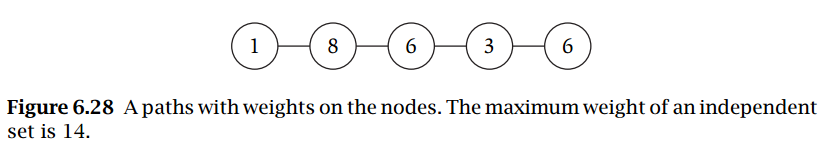
\includegraphics[scale=0.75]{1.PNG}

\vspace{2mm}

\noindent \textbf{(c)}  Give an algorithm that takes an n-node path G with weights and returns an independent set of maximum total weight. The running time should be polynomial in n, independent of the values of the weights.

\vspace{6mm}

\begin{lstlisting}
# G is an array of integers of length n, representing
# the ordered nodes of the path. G[i] is the weight of that node.
# returns an array containing the nodes in the largest
# independent set
find_set(G)
  S = empty array # will contain the independent set
  M = array[0 to n] # n = length of G
  M[0] = 0
  for i in [1 to n] # inclusive of ends
    if G[i]+M[i-2] > M[i-1]
      S.push_back(i) # push this (ith) node into our set
      M[i] = G[i]+M[i-2]
    else
      M[i] = M[i-1] # else we just use the last node
  return S
\end{lstlisting}

The subproblems that I'm solving are the ones involving the two previous nodes. At each node $i$, we can either take that node and not take its neighbor (by the rules of being independent set), or we can skip the current node and take its immediate neighbor. Thus we need to know which of these two subproblems results in a larger independent set in order to make the right choice. The subproblems are related in that if a node $i$ is in the largest independent set on a graph $G$, then neither of its neighbors can be in that set, so we don't have to consider those nodes. \\
The recurrance is $ f(n) = max(v_i+f(n-2), f(n-1)) : f(0) = 0 $. \\
We have an array to fill in as apposed to a table, this is because we are only working in a single variable, the iteration variable. We fill in the table from low to high index. The table is initialized with the 0th entry being set to zero, if there are no nodes to look at then we get no value from them. \\
An arrow diagram would point from node $i$ to the two nodes preceding it. \\
This algorithm is also linear on $n$, with it's running time being $O(n)$. This is just like the previous problem, even though our recurrance relation spaws many children, there are a large number of redundent calls being made. With memoization, we simply have to fill in the $n$ array values, starting from the first index and working our way up. On the way, we keep track of which items go into the final set by seeing which is the two options (M[n-1] or G[i]+M[i-2]) are larger, if it is the latter than we add node $i$ into the set. Because the algorithm iterates $n$ times and performs constant work each time, the running time is $O(n)$.


\end{homeworkProblem}





%----------------------------------------------------------------------------------------
%   PROBLEM 3
%----------------------------------------------------------------------------------------
\begin{homeworkProblem}

\vspace{2mm}

\noindent Let $G = (V, E)$ be a directed graph with nodes $v_1, ..., v_n$. We say that G is an ordered graph if it has the following properties. 

\vspace{2mm}

\textbf{(i)} Each edge goes from a node with a lower index to a node with a higher index. That is, every directed edge has the form $(v_i, v_j)$ with $i < j$. 

\vspace{2mm}

\textbf{(ii)} Each node except vn has at least one edge leaving it. That is, for every node $v_i$, $i = 1, 2, ..., n − 1$, there is at least one edge of the form $(v_i,v_j)$. 

\vspace{2mm}

The length of a path is the number of edges in it. The goal in this question is to solve the following problem (see Figure 6.29 for an example).

\vspace{2mm}

\emph{Given an ordered graph G, find the length of the longest path that begins at $v_1$ and ends at $v_n$.}

\vspace{2mm}

\noindent \textbf{(a)} Show that the following algorithm does not correctly solve this problem, by giving an example of an ordered graph on which it does not return the correct answer.

\begin{lstlisting}
Set w = v_1
Set L = 0

While there is an edge out of the node w 
  Choose the edge (w, v_j) 
    for which j is as small as possible 
  Set w = v_j   
  Increase L by 1 
end while 
Return L as the length of the longest path

\end{lstlisting}

\vspace{2mm}

In your example, say what the correct answer is and also what the algorithm above finds. \\[.2in]

\textbf{Answer :} 
This algorithm is too greedy, so all we need to do is trick it into picking a very close neighbor originally, and set it up so this neighbor only leads to a very short path between it and $v_n$. An example is given gelow.

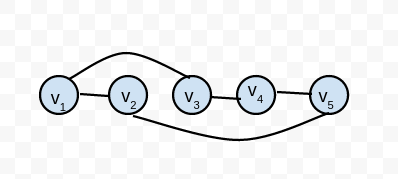
\includegraphics[scale=1]{graph1.png}

In the above graph, all edges are going left to right, my software wouldn't draw curved arrows so I just used lines. The algorithm given would start at $v_1$, and select the edge to $v_2$, since that is the closest vertex which is reachable directly. It will then be forced to take the single edge from $v_2$ to $v_5$, which finishes the algorithm with a score of 2. The optimal solution however would be to go from $v_1$ to $v_3$, $v_3$ to $v_4$, then $v_4$ to $v_5$, for a score of 3. \\[.2in]


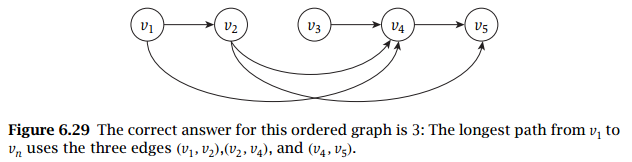
\includegraphics[scale=1]{2.PNG}

\vspace{2mm}

\noindent \textbf{(b)} Give an efficient algorithm that takes an ordered graph G and returns  the length of the longest path that begins at $v_1$ and ends at $v_n$.(Again, the length of a path is the number of edges in the path.) \\

\textbf{Answer :} This one took me a while to think about, because I was confused on what to concentrate on, the vertices or the edges. I ended up coming up with following notation : $$ E_i = \{ e_{i1} e_{i2} \ldots e_{ip} \} $$ the set of all edges that end at vertex $i$ ($i$ is the target). Each edge $e_{ik} \in E_i$ has a source labeled $e_{ik}.s$. \\

The sub-problems that we are worried about solving is finding the maximum length path from vertex 1 to any vertex that comes before the current vertex and has an edge connecting it to the current vertex. Thus for a given vertex $n$ with edge set $E_n$, we need to find the lengths of the longest path from the start vertex to all vertices that are the source of an edge in $E_n$. \\
The subproblems are related in that if we know the length of the longest path from the start to a vertex that is before the current one and connected to the current one, then the length of the longest path could be 1 + the length of the longest path to that vertex. To find the true longest path, we take the max of the longest paths to every previous vertex and add one. \\
The recurrance is $ f(i) = 1+max(f(k) : k = e.s $ $ \forall e $ $ \in E_i) $ and $f(1) = 0$. This says that we look at the longest path for all vertices before and adjascent to the current vertex, and add one to the max of these values. The base case is on the first vertex, there is no where to go so the longest path $f(1)=0$. \\
We once again only have an array to fill in as opposed to a table, because this problem only needs to memoize what is the best path for each of the $n$ vertices. The recursion states that the $n$th problem depends on all problems $i$ such that there is an edge $(i, n)$, so there would be arrows pointing backwards towards all adjascent vertices. The table is filled in algorithmically left to right, starting by filling in the first index with 0 and moving up, using the recurrance and the edge lists to fill in the individual sub-problems.  \\

My algorithm goes through all vertices, starting at the beginning, and fills in the memoization array using the recurrance defined above. One issue is that since this is a directed graph, natural graph representations don't know which edges point in to which vertices, only what points out. This means that for each iteration of the loop $i$, we have to go through each vertex $k < i$ and check if there is an edge $(k,i)$, one that points to the current vertex. If so we add the value of the max length for that vertex $k$ to a list, which we end up taking the max value from. This guarentees that we find the longest path to the current vertex, which must be 1 plus the maximum of the longest paths to all precending, adjascent vertices. \\

Note that this problem didn't ask to find the longest path, just the length, which simplifies the algorithm slighly by lessening the book-keeping.

\vspace{6mm}

\begin{lstlisting}
# G = adj. matrix representation of graph on n vertices [1 to n].
# G[i][k] = 1 if an edge from vertex i to vertex k, 0 otherwise
# returns an integer that gives the longest path length
find_longest_path(G)
  M = array[1 to n] # will hold max length vals for all sub-problems
  V = empty max heap # will hold temp. values for max function
  M[1] = 0
  for i in [1 to n] # inclusive of ends
    for j in [1 to i-1] # only go to current vertex, not passed
      if(G[j][i] == 1) #if edges from j to i
        V.insert(M[j]) # add the length value to the heap, note that because
                          # j < i, M[j] is defined.
    M[i] = 1 + max(V) # set length 1 + max length of all adjascent, preceding vertices
    V.empty() # clear the list for the next iteration

  return M[n]
\end{lstlisting}

The running time for this problem is $O(n^2logm)$, where $m$ is the maximum number of incoming edges from preceding vertices that a given vertex has in a specific graph. This is because for each incoming edge, we have to perform a heap insertion of the M value for that source vertex, which is logarithmic in the size of the heap. Note that $m$ is always bounded above by $n$, so this could be replaced by $O(n^2log(n))$ for a looser bound. The $n^2$ term comes from the faux double for loop, the outer one runs $n$ times and the inner one runs a variable number of times bounded by $n$.

\end{homeworkProblem}





%----------------------------------------------------------------------------------------
%   PROBLEM 4
%----------------------------------------------------------------------------------------
\begin{homeworkProblem}


\vspace{2mm}

\noindent In a word processor, the goal of ``pretty-printing'' is to take text with a ragged right margin, like this,

\vspace{2mm}

\begin{lstlisting}
Call me Ishmael. 
Some years ago, 
never mind how long precisely,
having little or no money in my purse, 
and nothing particular to interest me on shore, 
I thought I would sail about a little 
and see the watery part of the world.

\end{lstlisting}

\vspace{2mm}

\noindent and turn it into text whose right margin is as ``even'' as possible, like this.

\vspace{2mm}

\begin{lstlisting}

Call me Ishmael. Some years ago, never 
mind how long precisely, having little 
or no money in my purse, and nothing 
particular to interest me on shore, I 
thought I would sail about a little 
and see the watery part of the world.

\end{lstlisting}

\vspace{2mm}

To make this precise enough for us to start thinking about how to write a pretty-printer for text, we need to figure out what it means for the right margins to be ``even.'' So suppose our text consists of a sequence of words, $W={w_1,w_2,...,w_n}$, where $w_i$ consists of $c_i$ characters. We have a maximum line length of L. We will assume we have a fixed-width font and ignore issues of punctuation or hyphenation. 

A formatting of W consists of a partition of the words in W into lines. In the words assigned to a single line, there should be a space after each word except the last; and so if $w_j, w_{j+1}, ..., w_k$ are assigned to one line, then we should have 

\centerline{ $\displaystyle[\sum_{i = j}^{k - 1} (c_i + 1)] + c_k \le L.$
}

\noindent We will call an assignment of words to a line valid if it satisfies this inequality. The difference between the left-hand side and the right-hand side will be called the slack of the line—that is, the number of spaces left at the right margin. 

Give an efficient algorithm to find a partition of a set of words W into valid lines, so that the sum of the squares of the slacks of all lines (including the last line) is minimized.

\vspace{6mm}

\textbf{Answer :} \\
The sub-problems in this case are how the preceding groupings of words line-up given the line that you wish to put the current word on. In other words, if on the current word $w_i$ you decide to start a new line, whether or not this is optimal depends on if this newline disrupts the optimal solution of the preceding words. \\
The subproblems are related in that if we know how the various groupings of the preceding words are scored, we can see how we should best rearrange the lines to add in the current word by taking a min. over all possible previous word combinations. \\
To start, define Opt(i) to be the cost of the optimal way of arrange words $w_1$ through $w_i$, aka the minimized square slack over the first $i$ words.\\
The recurrence is then : $$ Opt(0) = 0 \text{ and }Opt(i) = \text{min}_{1\leq t \leq i}(Opt(t-1) + S[t][i]) $$ S[t][i] refers to a table entry that contains the slack associated with arranging words $t$ through $i$ into a single line. Notice that we take the minimum over all possible line arrangements of the preceding words to find which one to add the current word to. \\
I use two closely related tables to solve this problem. If there are $n$ words to be pretty-printed, the first table of values $T$ will be of size $n \times n$. The $T$[k][j] index will represent the number of characters by placing the words going from $w_k$ to $w_j$ on a single line. I then define a table $S$[i][j] of equal size the components of which are $ S_{ij} = (L - T_{ik})^2$ if $ T_{ik} \leq L $ and $\infty $ otherwise, this table represents the slack associated with grouping words $i$ through $j$ into a line. Finally, I also need an array Opt[j] which contains the total score associated with the optimal arrangement of the first $j$ words. By total score I mean the sum of the squared slacks of the lines used to arrange the first $j$ words. \\

The algorithm is given below, it relies on the \verb.generate_table. subroutine which is defined below that. Instead of taking in a list of words in their entirety, it's easier to just get a list of integers representing the word length. Thus the algorithm is given a vector of word lengths (integers greater than zero), and a maximum line length L. The function will return a list of indices representing the words that are at the start of each line. Knowing these words is enough to define the entire structure of the document. Also note that even though the recurrance says we need to take the minimum over all sized groupings of words from 1 to $i$, we really only need to look backwards from $i-1$ until we find a sequence which is longer than L, we can stop because going further back (making a longer sequence of words) will only result in a sequence which also doesn't fit on a line. P is an array that, in index $i$ stores the first word on the last line of the optimal arrangement for words 1 to $i$. At the end of the algorithm, we will parse this array to get the final array of words that start each line by starting at $P_n$ and working our way backwards.

\begin{lstlisting}
# W = vector of n word lengths [w1 to wn]
# L = max line length (> 0)
pretty_print(W, L)
S = generate_table(W, L)
n = W.size() # number of words is our iteration count
Opt = empty array[1 to n]
P = empty array[1 to n] 
Opt[1] = 0
for i in 1 to n
  Opt[i+1] = integer::max # equiv. of infinity
  t = i
  Temp = Opt[t] + S[t, i]
  while t > 1 and Temp < integer::max # look backwards at larger sets of words
    Temp = Opt[t-1] + S[t-1, i] # recurrence
    if Temp < Opt[i+1]
      Opt[i+1] = Temp
      P[i] = k # k is best choice for words 1 to i

# extract the true starting words from the P array
ret = empty list
i = n
ret.insert(P[--i])
while i > 0
  ret.insert(P[i])
  i -= P[i] # get the best solution for all words before P[i]

return ret

\end{lstlisting}

\newpage
\end{homeworkProblem}






%----------------------------------------------------------------------------------------
%   PROBLEM 5
%----------------------------------------------------------------------------------------
\begin{homeworkProblem}


\vspace{2mm}

\emph{Gerrymandering} is the practice of carving up electoral districts in very careful ways so as to lead to outcomes that favor a particular political party. Recent court challenges to the practice have argued that through this calculated redistricting, large numbers of voters are being effectively (and intentionally) disenfranchised. 

Computers, it turns out, have been implicated as the source of some of the ``villainy'' in the news coverage on this topic: Thanks to powerful software, gerrymandering has changed from an activity carried out by a bunch of people with maps,pencil,and paper into the industrial-strength process that it is today. Why is gerrymandering a computational problem? There are database issues involved in tracking voter demographics down to the level of individual streets and houses; and there are algorithmic issues involved in grouping voters into districts. Let's think a bit about what these latter issues look like. 

Suppose we have a set of n precincts $P1, P2, ..., Pn$, each containing m registered voters. We're supposed to divide these precincts into two districts, each consisting of $n/2$ of the precincts. Now, for each precinct, we have information on how many voters are registered to each of two political parties. (Suppose, for simplicity, that every voter is registered to one of these two.) We'll say that the set of precincts is susceptible to gerrymandering if it is possible to perform the division into two districts in such a way that the same party holds a majority in both districts.

Give an algorithm to determine whether a given set of precincts is susceptible to gerrymandering; the running time of your algorithm should be polynomial in $n$ and $m$. 

\vspace{2mm}

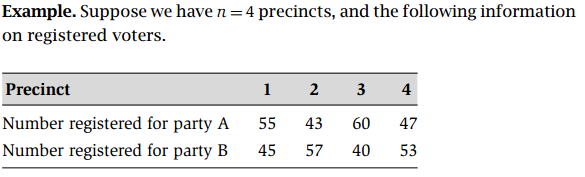
\includegraphics[scale=0.75]{3.PNG}

\vspace{2mm}

This set of precincts is susceptible since, if we grouped precincts 1 and 4 into one district, and precincts 2 and 3 into the other, then party A would have a majority in both districts. (Presumably, the ``we'' who are doing the grouping here are members of party A.) This example is a quick illustration of the basic unfairness in gerrymandering: Although party A holds only a slim majority in the overall population (205 to 195), it ends up with a majority in not one but both districts.

\vspace{6mm}


\end{homeworkProblem}






%----------------------------------------------------------------------------------------
%   PROBLEM 6
%----------------------------------------------------------------------------------------
\begin{homeworkProblem}


\vspace{2mm}

Recall the scheduling problem from Section 4.2 in which we sought to minimize the maximum lateness. There are $n$ jobs, each with a deadline $d_i$ and a required processing time $t_i$, and all jobs are available to be scheduled starting at time $s$. For a job $i$ to be done, it needs to be assigned a period from $s_i \ge s$ to $f_i = s_i + t_i$, and different jobs should be assigned nonoverlapping intervals. As usual, such an assignment of times will be called a schedule. 

In this problem, we consider the same setup, but want to optimize a different objective. In particular, we consider the case in which each job must either be done by its deadline or not at all. We'll say that a subset J of the jobs is schedulable if there is a schedule for the jobs in J so that each of them finishes by its deadline. Your problem is to select a schedulable subset of maximum possible size and give a schedule for this subset that allows each job to finish by its deadline. 

\vspace{2mm}

\noindent \textbf{(a)} Prove that there is an optimal solution $J$ (i.e., a schedulable set of maximum size) in which the jobs in $J$ are scheduled in increasing order of their deadlines. 

\vspace{2mm}

\noindent \textbf{(b)} Assume that all deadlines $d_i$ and required times $t_i$ are integers. Give an algorithm to find an optimal solution. Your algorithm should run in time polynomial in the number of jobs $n$, and the maximum deadline $D = max_i d_i$. 


\end{homeworkProblem}



%----------------------------------------------------------------------------------------

\end{document}